\chapter{Introducción}
\label{cap:Introduccion}

\section{Motivación}
\label{sec:Motivacion}
En los últimos años, la Ingeniería del Software ha observado notables cambios a la hora de desarrollar proyectos software. Tradicionalmente, el modelo de desarrollo de software utilizado consistía en la coordinación de diferentes equipos de trabajo en un mismo edificio (\emph{Desarrollo Colocalizado}), posteriormente, estos equipos de trabajo pasaron a organizarse entre diferentes edificios de una o varias ciudades, pero siempre centralizados en un mismo país (\emph{Desarrollo Distribuido}). Sin embargo, en la actualidad y debido a la globalización, cada vez más compañías separadas geográficamente colaboran para desarrollar software hasta traspasar fronteras llegando a un nivel mundial, por lo que se ha evolucionado hacia un modelo de desarrollo mucho más globalizado y deslocalizado, conocido como \emph{Desarrollo Global de Software} (DGS), o en inglés \emph{Global Software Development} (GSD) \cite{piattini2014desarrollo}.

El DGS está teniendo cada vez más aceptación entre los profesionales. Esta tendencia consiste en la colaboración entre diferentes equipos de desarrollo (fig.~\ref{fig:DGSFiguraMapa}), los cuales se encuentran ubicados alrededor del mundo en diferentes ciudades, países y continentes. Estos grupos de trabajo pueden pertenecer a distintas organizaciones, pero trabajan conjuntamente en un mismo proyecto software. En el proyecto podrá existir tanto una comunicación \emph{asíncrona} como \emph{síncrona} entre los equipos de trabajo, lo cual dependerá de una serie de características del proyecto \cite{prikladnicki2008improving}. 

\begin{figure}[htb]
	\centering
	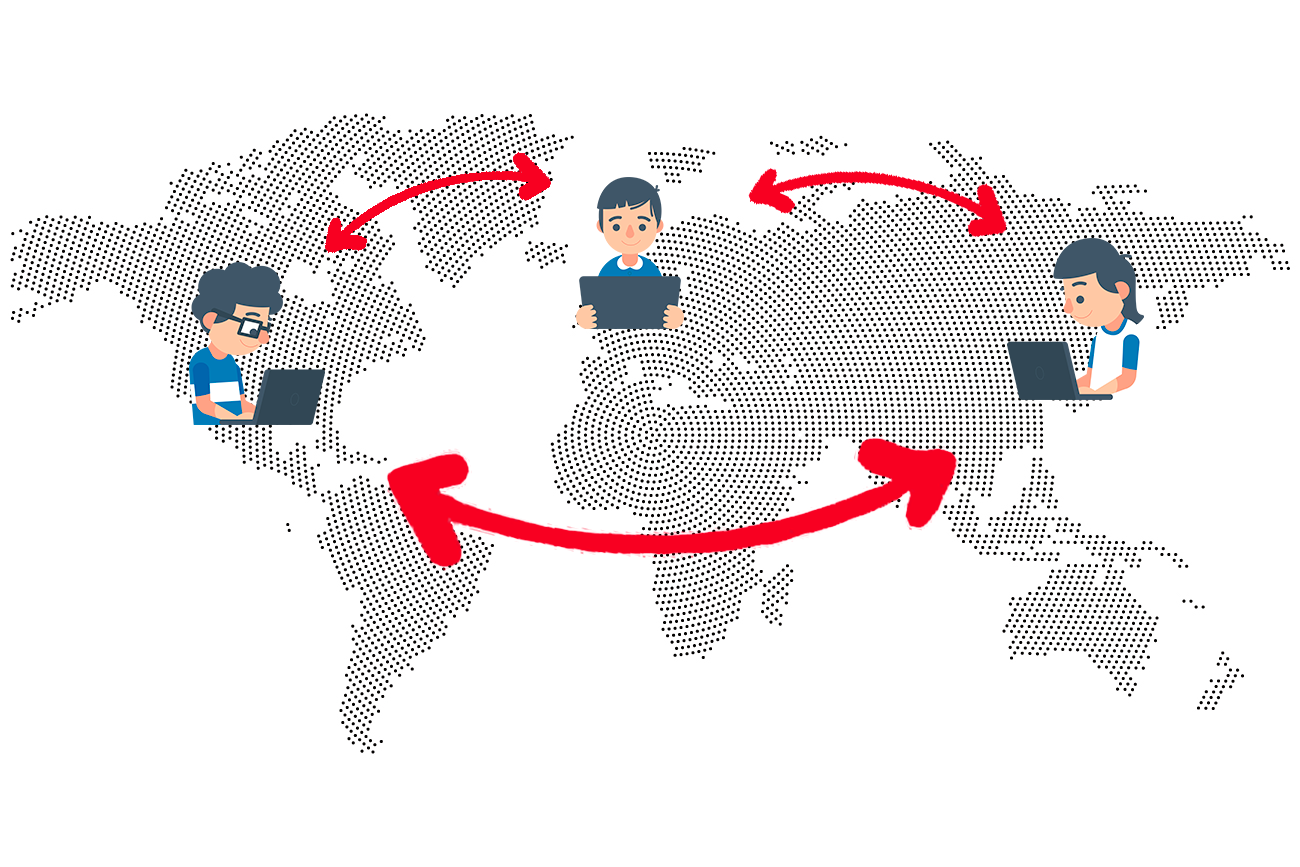
\includegraphics[width=0.75\linewidth]{DGSFiguraMapa}
	\caption[Colaboración mundial en el DGS]{En el DGS diferentes equipos de desarrollo colaboran a nivel mundial en un mismo proyecto}
	\label{fig:DGSFiguraMapa}
\end{figure} 

Gradualmente, esta tendencia esta cogiendo cada vez más fuerza en el campo de la ingeniería del software, considerándose una norma en el desarrollo de software \cite{bosnic2019assessing}. Esto es debido a que las organizaciones pueden conseguir grandes beneficios utilizando este nuevo modelo de desarrollo, ya que la principal ganancia que se consigue con su uso es la reducción en el coste económico de los proyectos, debido a que se suelen buscar territorios donde la mano de obra cualificada es barata y fácilmente disponible \cite{monasor2010preparing}. Además, se pueden encontrar otros beneficios notables como pueden ser el acercamiento del desarrollo del software al cliente y al mercado local, la reducción del período necesario para el desarrollo del software al maximizar la productividad y la expansión hacia la inclusión de trabajadores mayormente cualificados en sus actividades de desarrollo \cite{aagerfalk2008benefits}.

Sin embargo, acompañando a las anteriores ventajas que se pueden conseguir con los proyectos DGS, existen una serie de inconvenientes, los cuales son causados, principalmente, a las diferencias existentes en este tipo de proyectos las cuales podemos dividir en cuatro clases: las \emph{diferencias lingüísticas}, la \emph{distancia geográfica}, la \emph{diferencia cultural} y la coexistencia de diferentes \emph{zonas horarias}; haciendo mucho más difícil el consenso y entendimiento común \cite{monasor2010preparing}. Estas diferencias acentúan la problemática de administrar y gestionar un proyecto software, apareciendo así los tres principales desafíos en la gestión de proyectos DGS (fig.~\ref{fig:desafiosDGS}), también llamado en \cite{piattini2014desarrollo} como las 3 ces:
\begin{itemize}
	\item Desafíos en la comunicación. Los equipos de trabajo deben mantener una comunicación adecuada y activa, con el fin de llevar a cabo un intercambio constante de información y conocimientos. 
	\item Desafíos en la coordinación. Las tareas deben estar sincronizadas, para no sufrir retrasos y alcanzar objetivos e intereses comunes. 
	\item Desafíos en el control. El proyecto debe ser gestionado constantemente y confirmar que se cumplen fechas de entrega, estándares, presupuestos, etc.; además de solventar posibles contratiempos que puedan ocurrir durante el ciclo de vida del proyecto. 
\end{itemize}

\begin{figure}[htb]
	\centering
	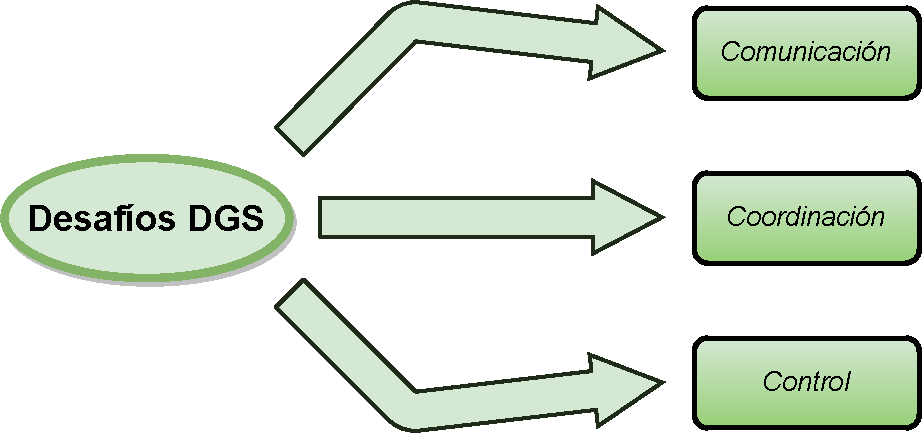
\includegraphics[width=0.75\linewidth]{desafiosDGS}
	\caption[Desafíos en los proyectos DGS]{Los tres principales desafíos en la gestión de proyectos DGS}
	\label{fig:desafiosDGS}
\end{figure}

Estos inconvenientes y desafíos complican la gestión de este tipo de proyectos, lo que puede implicar en retrasos de tareas o incluso en la cancelación del mismo, ya que según la literatura, la mayoría de proyectos DGS terminan fracasando. Según \cite{lino2015project}, la principal causa del elevado fracaso de estos proyectos es debido a la imperfecta y dificultosa gestión de los mismos. Es por esto, que para conseguir los beneficios que nos ofrece el DGS es necesario que los jefes de proyecto posean grandes conocimientos y experiencia en la gestión de estos proyectos, además de contar con una serie de habilidades (no solo técnicas, sino también no técnicas), para hacer frente a los posibles contratiempos que puedan ocurrir en el ciclo de vida del proyecto y conseguir la finalización exitosa del mismo.


\section{Propuesta}
\label{sec:Propuesta}

\section{Estructura del documento}
\label{sec:Estructura}